\chapter{Wprowadzenie teoretyczne}
\label{cha:wprowadzenieTeoretyczne}

\section{Dobór odpowiedniej metodologii}
\label{sec:doborMetodologi}

Tworząc aplikację internetową pierwszym i prawdopodobnie najważniejszym krokiem
jest dobranie metodologii wytwarzania oprogramowania oraz ogólnych praktyk, które
należy stosować. Obecnie dwa najpopularniejsze podejścia do zarządzania projektem
praktykowane w przedsiębiorstwach to model kaskadowy (ang. waterfall) oraz model
zwinny (ang. agile).

\subsection{Model kaskadowy}
\label{subsec:modelKaskadowy}
Podejście waterfall jest klasycznym systemem używanym w wielu branżach,
polegającym na wyszczególnieniu konkretnych faz projektowych, następujących kolejno po sobie. W
przypadku projektów informatycznych fazy te są następujące: faza koncepcyjna, rozpoczęcie,
analiza, projektowanie, budowa, testy, produkcja/wdrożenie oraz obsługa. Główne
założenia tego modelu to: szczegółowy plan, sekwencyjna realizacja zadań, rygorystyczne
przestrzeganie terminów oraz konsekwentne prowadzenie dokumentacji. Zalety tego
podejścia to między innymi określenie bardzo szczegółowych wymagań klienta na początku
całego procesu, jasno określone rezultaty oraz zmniejszone prawdopodobieństwo
nieporozumień wewnątrz zespołu, bądź na linii klient-realizator. Model ten posiada jednak
kilka wad takich jak brak możliwości powrotu do wcześniejszej fazy oraz 
modyfikacji wymagań klienta podczas rozwoju aplikacji, możliwość przeprowadzenia
fazy testowania dopiero pod koniec procesu, co wiąże się z dodatkowymi kosztami na wielu
poziomach. Na podstawie wyżej wymienionych zalet oraz wad można wysnuć wnioski, że
model ten nadaje się do realizacji projektów o jasno określonych wymaganiach, gdzie
dokładność jest ważniejsza niż szybkość wykonania. Niestety obecnie w obszarze tworzenia
oprogramowania coraz częściej pojawiają się dynamicznie zmieniające się wymagania klientów, dużą konkurencje, niestabilny rynek, brak jednolitych standardów i regulacji przez
co model ten wydaje się przestarzały, ryzykowny i nieopłacalny.
\subsection{Model zwinny}
\label{subsec:modelZwinny}
W odpowiedzi na potrzeby zespołów programistów w 2001 roku powstał koncept
podejścia zwinnego. Jego założenia były zupełnie inne niż w przypadku podejścia
kaskadowego. Indywidualności oraz interakcje zamiast procesów i narzędzi, działające
oprogramowanie zamiast obszernej dokumentacji, bezpośrednia i stała współpraca z klientem
zamiast negocjacji kontraktu, odpowiedź na zmienne wymagania zamiast podążania za z góry
wytyczonym planem \cite{MAN01}. Dziś podejście agile nie jest uważane za konkretną metodologię,
a raczej za zbiór pomysłów, które można stosować w wielu kombinacjach, dostosowanych do
potrzeb projektu oraz zespołu.


Nowoczesne, zwinne podejście opiera się na pięciu zasadach\cite{AGI01}. Pierwszą z nich jest
jasno zdefiniowana rola menadżera, dewelopera, klienta oraz zespołu. Zespół jako całość ma
obowiązek podziału zadań do wykonania oraz przydzielania ich do poszczególnych członków zespołu. Rola
klienta natomiast nie sprowadza się do bycia pasywnym, lecz staje się on aktywnym
uczestnikiem procesu wytwarzania oprogramowania. Drugą zasadą jest odrzucenie wymagań
oraz fazy projektowania na początku procesu, ponieważ klient nie może w 100 procentach wiedzieć czego dokładnie chce i
nie jest w stanie tego określić na takim etapie. Zamiast tego stosowana jest ciągła współpraca
z klientem, który dynamicznie ustala swoje wymagania co do produktu. Następną zasadą jest
stosowanie iteracji. Na początku każdej iteracji określane są jej wymagania oraz lista
funkcjonalności do zaimplementowania. Każda iteracja trwa małą, określoną ilość czasu oraz
zakłada brak dodawania wymagań podczas tego okresu. Krótki czas zmniejsza również
koszty związane z implementacją funkcjonalności, które mogą stać się nieaktualne pod koniec
iteracji. Kolejnym dogmatem jest ograniczenie niepotrzebnej funkcjonalności. Oznacza to, że
każda funkcjonalność ma określoną wartość biznesową, dzięki czemu zespół nie
implementuje czegoś, co nie będzie nigdy użyte w końcowym produkcie. Dodatkowo ustala
się potencjalny czas wykonania danej funkcjonalności w celu lepszego przydzielenia zadań na
iterację. Ostatnia zasada skupia się na jakości wytwarzanego oprogramowania. W metodach
zwinnych jest ona uzyskiwana poprzez ciągłe testowanie na przestrzeni całego procesu
tworzenia produktu. Aby funkcjonalność została zaakceptowana i wdrożona na produkcję
musi przejść wszystkie testy.

\section{Dobór odpowiednich technik wytwarzania oprogramowania}
\label{sec:doborTechnikWytwarzania}

Wydawało by się, że metodologia zwinna nadaje się do każdego projektu
informatycznego, jednak praktyka na przestrzeni wielu lat pokazała, że są one często
nadinterpretowane bądź potencjalna wartość dodana stosowanej praktyki jest mocno
zawyżona. W rzetelnej analizie najpopularniejszych technik zwinnych nieocenioną pomocą
okazały się publikację Bertranda Meyera oraz Lecha Madeyskiego. Pierwsza pozycja odnosi się do tez głoszonych przez
autorytety w dziedzinie inżynierii oprogramowania dotyczących metodyki zwinnej oraz ocenia powszechnie stosowane
metody, opierając się na wieloletnim doświadczeniu zdobytym przez programistów\cite{AGI01}. Druga
opisuje badania przeprowadzone na studentach Politechniki Wrocławskiej, które dotyczą
dwóch najbardziej popularnych praktyk czyli Pair Programming oraz Test-Driven
Development\cite{TDD01}. Eksperyment miał pokazać wpływ wyżej wymienionych praktyk m.in. na testy
akceptacyjne, stopień powiązania ze sobą nowo utworzonych klas, pokrycie kodu testami
jednostkowymi oraz liczbę defektów. Po zapoznaniu się z obiema pozycjami można wyróżnić
kilka technik, które wydają się być najbardziej odpowiednie dla realizowanego projektu.

\subsection{Krótkie iteracje}
\label{subsec:krótkieIteracje}

Wspomniane wcześniej krótkie iteracje oraz wiążące się z nimi zamknięcie się na
jakiekolwiek dodawanie nowych funkcjonalności w ich obrębie, brak opóźnień pomimo nie
wykonania wszystkich zadań oraz skupienie się na dostarczeniu działającego oprogramowania na koniec każdej z nich są prawdopodobnie najważniejszymi praktykami
wprowadzonymi przez podejście zwinne. Wielu specjalistów docenia je ze względu na
częste punkty kontrolne podczas procesu produkcji oprogramowania oraz możliwość
otrzymania niemal natychmiastowej informacji zwrotnej od klienta. Brak opóźnień w iteracji
wraz z zamknięciem się na zmianę wymagań sprawiają, że nic nie zakłóca pracy i programista
jest w stanie bardziej skupić się na konkretnym zadaniu. Dodatkową zaletą jest większy czas na określenie wartości biznesowej danego pomysłu przez klienta, dzięki czemu może
lepiej sprecyzować swoje zapotrzebowania. W przypadku projektu, w którym wymagania będą
się zmieniały bardzo dynamicznie najlepszym wyborem jest 14 dniowy okres jednej iteracji,
ponieważ gwarantuje to możliwość modyfikacji założeń lub wymagań w bardzo krótkim
czasie, co wydaje się kluczowe podczas mocno ograniczonego czasu na wykonanie projektu.

\subsection{Faza projektowania i ustalenia wymagań}
\label{subsec:fazaProjektowania}

Następną, mocno kontrowersyjną praktyką jest odrzucenie wymagań oraz fazy
projektowania na początku procesu. Nie można zaprzeczyć, że określenie wszystkich
potrzebnych wymagań na początku jest niemożliwe. Wraz z postępami architektura systemu
również będzie wielokrotnie zmieniana, dlatego teoretycznie z biznesowego punktu widzenia
faza projektowania jest nieopłacalna. Z drugiej strony wnikliwe przestudiowanie problemu
przed próbą rozwiązania go znacząco poprawia początkową pracę zespołu, dlatego
doświadczeni inżynierowie nie pomijają tego kroku\cite{AGI01}. Jednak w przeciwieństwie do założeń
modelu kaskadowego, wymagania ustalone podczas fazy projektowania powinny być
traktowane jak każdy inny artefakt, czyli ulegać zmianie wraz z postępem prac.
Dodatkowo jakiekolwiek wymagania nie powinny się składać tylko i wyłącznie ze
scenariuszy użytkownika systemu, ponieważ nie pokazują one abstrakcji różnych
komponentów. Opierając się tylko na nich programista nie jest w stanie stworzyć funkcjonalności
łatwych do zaadaptowania w nowych przypadkach. Wymienione scenariusze powinny być
uzupełnieniem wymagań, potwierdzać ich kompletność. Biorąc pod uwagę wszystkie
argumenty za i przeciw można wysnuć wniosek, że przeprowadzenie fazy projektowania i
ustalenia wstępnych wymagań w celu zaprojektowania ogólnej architektury projektu oraz
zdefiniowania funkcjonalności aplikacji jest krokiem koniecznym. Jednak zgodnie z
podejściem zwinnym ustalenia te będą się zmieniały.

\subsection{Test-Driven Development}

Często stosowaną aczkolwiek kontrowersyjną praktyką jest Test-Driven Development. Jej
najpopularniejsza definicja\cite{TDD04} mówi, że jest to technika tworzenia oprogramowania, polegająca
na pisaniu testów przed napisaniem kodu. Jest ona jednak niekompletna, ponieważ opisuję
tylko część Test-First, nie skupiając się na głównych jej założeniach oraz fazach. W TDD
możemy wyróżnić trzy główne fazy każdego cyklu tworzenia kodu. Pierwsza to faza Red,
która polega na napisaniu wszystkich możliwych testów dotyczących niezaimplementowanej
jeszcze funkcji. Na tym etapie żaden z testów nie powinien przejść. Faza ta pozwala na
dłuższe zastanowienie się nad tym jak dana funkcja ma wyglądać oraz jak ma się
zachowywać w określonych przypadkach. Następnie wyróżniamy fazę Green, która polega na
zaimplementowaniu funkcji tak, aby przeszła wszystkie napisane wcześniej testy. Jej
głównym celem jest znalezienie rozwiązania problemu bez skupiania się na optymalizacji i
jakości pisanego kodu. Ostatnią fazą jest Refactor, w której należy zastanowić się, jak
poprawić napisany wcześniej kod lub testy. Jest to prawdopodobnie najważniejsza część
TDD. Dzięki niej wzrasta jakość napisanego kodu oraz następuje optymalizacja rozwiązania
w wyniku czego nasz kod osiąga ostateczną formę.

\begin{figure}[h!]
	\makebox[\textwidth][c]{
		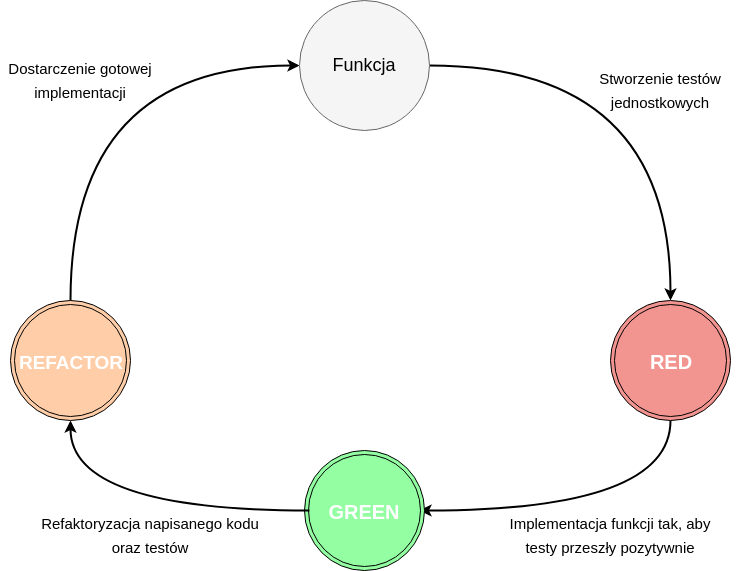
\includegraphics[width=\textwidth]{FazyTDD}
	}
	\caption{Proces implementacji funkcji w podejściu Test-Driven Development. }
	\centering
	\label{fig:TDD}
\end{figure}


Podejście zwinne jest przede wszystkim chwalone za powiązanie każdej
funkcjonalności z testami pozwalającymi na łatwą identyfikację błędów w późnych fazach
tworzenia projektu. Jeszcze ważniejsze jest postawienie na pierwszym miejscu refaktoryzacji
stworzonego kodu. Każdorazowa refleksja nad działaniem kodu, jego czytelnością i ogólnym
projektem sprawia, że inny programista jest w stanie go bez problemu zrozumieć, a projekt
może być rozwijany przez lata. Mimo, że TDD łączy te dwie, powszechnie uznane praktyki,
stosowanie go ma też swoje wady.


Pierwsze z nich dotyczą czasu wytwarzania oprogramowania oraz ogólnej
produktywności programisty. Każdorazowe stosowanie cyklu Red-Green-Refactor podczas
implementacji funkcji może znacząco wydłużyć czas wykonania projektu, jednak wszystko
zależy od stopnia złożoności problemu oraz od umiejętności z zakresu pisania testów\cite{TDD02}.
Wydłużony czas tworzenia oprogramowania ma też w małym stopniu negatywny wpływ na
produktywność programisty. Kolejnym aspektem są problemy pojawiające się przy
korzystaniu z TDD przez osoby o niskich umiejętnościach programistycznych. Badania
przeprowadzone studentach\cite{TDD01} pokazały, że wraz ze wzrostem złożoności pojawia się problem z
pokryciem przez testy wszystkich przypadków, ich jakość jest niższa oraz często zmieniające
się wymagania powodują nieaktualność części napisanych testów. Zaobserwowano również
sporadyczne nieporozumienia między programistą, a testerem oprogramowania. Ponadto w
wielu publikacjach pojawia się stwierdzenie, że w praktyce inżynierowie często źle
wykonują poszczególne fazy procesu lub pomijają najważniejszą z nich czyli Refactor.


Z drugiej strony TDD posiada wiele zalet. Najważniejszą zaletą jest poprawa jakości
napisanego kodu\cite{TDD03}. Z przeprowadzonych badań\cite{TDD01} wynika, że w
porównaniu do podejścia Test-Last, Test-First ma znaczny, pozytywny wpływ na stopień
powiązań między klasami oraz na pokrycie testami. Dodatkowo z wewnętrznej obserwacji
firm stosujących tę technikę wynika, że ma ona pozytywny wpływ na liczbę defektów oraz
nieznaczny wpływ na procent pozytywnych testów akceptacyjnych. Inną zaletą, która często
się pojawia jest pozytywny wpływ na rozwój programisty i jego nawyków. W podejściu
Test-Last programista często pomija krok pisania testów, bądź nie przykłada do niego
wystarczająco dużo uwagi, co ma negatywny wpływ na projekt późnych fazach produkcji.
Test-Driven wymusza pewną samodyscyplinę w tym aspekcie oraz spojrzenie na
rozwiązywany problem z wielu perspektyw, co może powodować większy rozwój
umiejętności programowania.

Po przeanalizowaniu wszystkich argumentów za i przeciw pod kątem specyfiki
tworzonego projektu postanowiono wykorzystać pewne założenia Test-driven, jednak nie spełniać ich w stu procentach. Głównym powodem stojącym za tą decyzją jest ograniczony czas na stworzenie gotowego produktu. W przypadku braku dużego doświadczenia w pisaniu testów jednostkowych, integracyjnych, automatycznych czas ten znacznie się wydłuża. Jednocześnie postanowiono stosować fazę Refactor oraz pisanie testów dla najważniejszych elementów systemu.
\subsection{Planning poker}
\label{subsec:planningPoker}
Jest to technika wywodząca się z podejścia \textit{Scrum}, mająca za zadanie ułatwić proces estymacji kosztu wyprodukowania danej funkcjonalności. Polega ona na przydzieleniu poszczególnym \textit{User stories} punktów o nazwie \textit{Story points}, które mają symbolizować koszt związany z danym \textit{story}. W ramach tej techniki muszą zostać spełnione poniższe założenia\cite{AGI01}:
\begin{itemize}
\item poleganie na kolektywnym osądzie całego zespołu
\item przeprowadzanie iteracji do momentu uzyskania zgody wszystkich członków zespołu
\item unikanie niepotrzebnego przestoju wynikającego z małych różnic, dzięki ustaleniu ciągu liczb, którymi można określić \textit{Story points}
\end{itemize}

Najczęściej wybieranym ciągiem liczb jest ciąg Fibonacciego, czyli wartości \mbox{0, 1, 2, 3, 5, 8, 13, 21, ...} . Jeżeli estymacja symbolizuje ilość dni, które dana osoba musi przeznaczyć na wytworzenie danej funkcjonalności, wtedy często dodaje się wartość 0.5, która oznacza mniej niż jeden dzień. Zaletą tego podejścia jest uniknięcie niepotrzebnych dyskusji w zespole, które wynikałyby z nieznaczących różnic w wartościach np. między 11 a 12. Dodatkowo wybór musi być zgodny i zatwierdzony przez wszystkich członków zespołu, niezależnie od doświadczenia. Dzięki temu występuje małe prawdopodobieństwo niedoszacowania lub przeszacowania kosztu funkcjonalności oraz każda opinia zostaje wzięta pod uwagę.

Proces przydzielania punktów odbywa się z udziałem całego zespołu, właściciela produktu oraz klienta. Następnie wykonywane są następujące kroki:
\begin{enumerate}
	\item Jedna z osób opisuje wybraną funkcjonalność, najczęściej jest to właściciel produktu
	\item Następnie wszyscy uczestnicy dyskutują nad nią, zadają odpowiednie pytania, wymieniają się spostrzeżeniami
	\item Każdy wybiera wartość symbolizującą koszt wyprodukowania, wartość ta musi być zgodna z ustalonym wcześniej ciągiem
	\item Wszystkie wybory uczestników zostają przedstawione całej grupie
	\item Jeżeli wartości się zgadzają proces zostaje zakończony, a dana funkcjonalność jest już oceniona
	\item Jeżeli wartości nie są identyczne uczestnicy dalej dyskutują, po czym przechodzi się znów do kroku 3
	\item Jeżeli przez dłuższy czas nie można dojść do porozumienia należy porzucić daną historyjkę do czasu uzyskania nowych informacji i przejść do następnej
\end{enumerate}  

Po określeniu kosztu wszystkich historyjek, można przydzielić je do kolejnej iteracji. Aby zrobić to sprawnie i rzetelnie ustala się zdolność zespołu na danych sprint za pomocą już wspomnianych \textit{Story points}. Najczęściej wylicza się średnią osiągniętych punktów z ostatnich kilku iteracji. W przypadku pierwszej ustala się ją orientacyjnie i weryfikuje wraz z kolejnymi iteracjami. Następnie przydziela się dane historyjki tak, aby nie przekraczały zdolności zespołu. Dodatkowo można orientacyjnie wyliczyć ile czasu oraz iteracji zajmie stworzenie wszystkich funkcjonalności, jednak wraz ze zmieniającymi się wymaganiami oraz nowymi wymogami oszacowanie to traci na znaczeniu. 



\section{Wykorzystywane oprogramowanie}
\label{sec:wykorzystywaneOprogramowanie}
Do zaimplementowania platformy ProjectSHARE został użyty stos technologiczny składający się z popularnych szkieletów do budowy aplikacji tj. Spring framework oraz Angular 6. Spring został użyty w celu stworzenia REST API służącego do zarządzania zasobami, natomiast Angular w wersji 6 został wykorzystany do stworzenia warstwy prezentacji w postaci strony SPA (ang. Single-Page Application). Użyto również szkieletu Hibernate do realizacji warstwy dostępu do bazy danych PostgreSQL. W procesie zarządzania budową aplikacji na szkielecie Spring wykorzystane zostało narzędzie Apache Maven.

\subsection{Spring framework}
\label{subsec:springFramework}

W celu zaimplementowania logiki biznesowej w postaci REST API wykorzystano szkielet do budowy aplikacji (ang. framework) Spring, który mocno ułatwia tworzenie aplikacji biznesowych w języku programowania Java. Powstał on w 2003 roku, w swoich założeniach miał być uzupełnieniem bardzo skomplikowanej i złożonej specyfikacji Java EE \cite{SPR03}. W swoim działaniu używa kilka technologii Java EE takich jak Servlet API, WebSocket API, Bean Validation, JPA, JMS. Z czasem jego możliwości znacznie się powiększyły dzięki wprowadzeniu autorskich rozwiązań\cite{SPR02} np. Spring Boot, Spring MVC, Spring REST Spring Security, Spring Data. Jego główną zaletą jest ogromny wybór modułów oraz całkowita dowolność ich doboru w zależności od potrzeb. Ta elastyczność pozwala na stworzenie klarownej architektury dla wielu rodzajów aplikacji. Dodatkową zaletą tego szkieletu jest model open-source oraz wynikająca z tego ogromna społeczność, która w dużym stopniu pomaga go rozwijać. 

\begin{figure}[h!]
	\makebox[\textwidth][c]{
	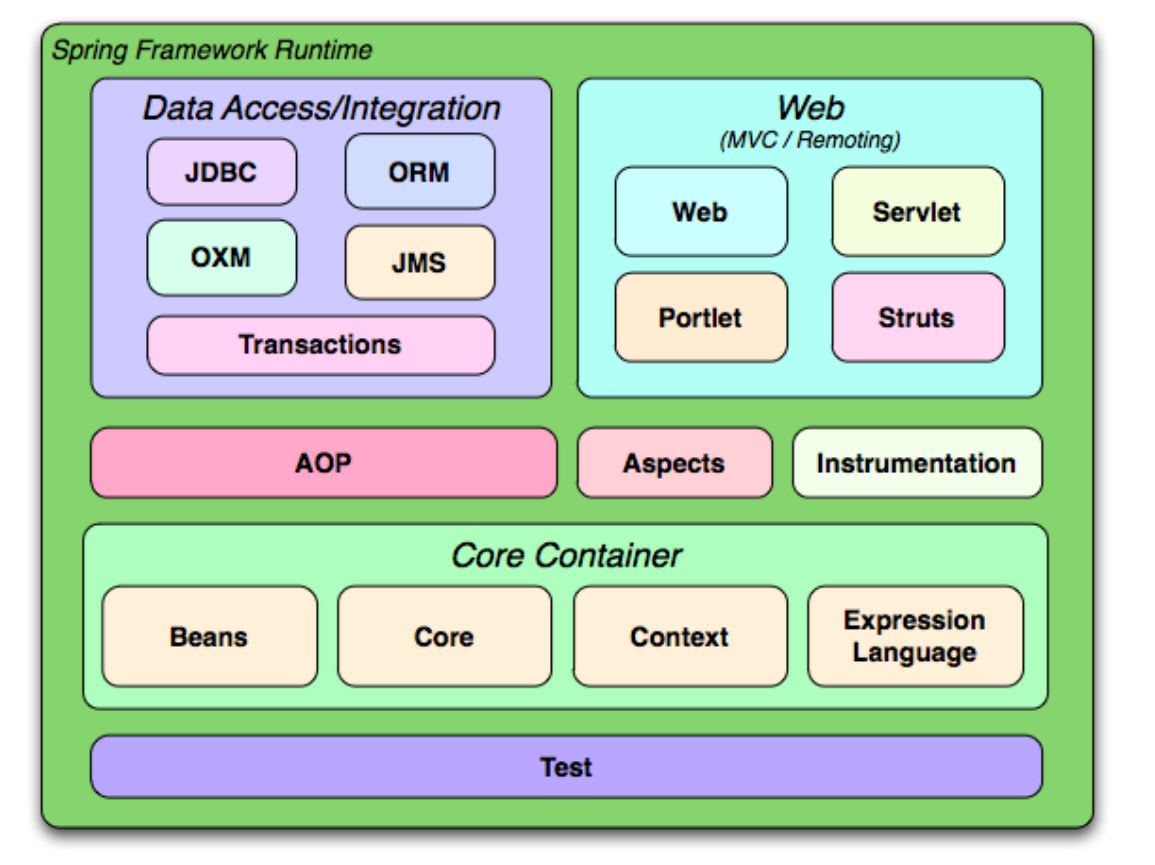
\includegraphics[width=\textwidth]{SpringStructure}
	}
	\caption{Uproszczona Struktura Spring framework. }
	    \caption*{Źródło: Spring framerwork Reference Docummentation}
	\centering
	\label{fig:springStructure}
\end{figure}


Strukturę Spring najłatwiej przedstawić jako ogromny zbiór konkretnych rozwiązań, każde z nich to osobny moduł, który można wykorzystać\cite{SPR01}. Pozwala to na zmianę projektu aplikacji na każdym etapie jej produkcji np. poprzez określenie innej implementacji za pomocą konfiguracji. Rdzeniem całego szkieletu oraz każdej aplikacji jest \textit{Core Container}, który zawiera najważniejsze moduły: \textit{Beans, Core, Context oraz Expression Language}. Moduły \textit{Core} oraz \textit{Beans} zapewniają najważniejsze mechanizmy, czyli wstrzykiwanie zależności (ang. \textit{Dependency Injection}) oraz wiążący się z nim wzorzec architektury odwrócenie sterowania (ang. \textit{Inversion of Control}). Odpowiadają również za całą logikę związaną z ziarnami (ang. beans) czyli klasami, które zostały odpowiednio adnotowane lub skonfigurowane. Ich instancjonowaniem zajmuje się klasa implementująca interfejs \textit{BeanFactory}, co pozwala na oddzielenie konfiguracji zależności od jej specyfikacji. Zadaniem modułu \textit{Context} jest zapewnienie dostępu do obiektów w sposób podobny do specyfikacji JNDI. Opiera się on na wspomnianych już modułach \textit{Core} oraz \textit{Beans}, wspiera również standardy Java EE takie jak np. EJB. Ostatnim modułem jest \textit{Expression Language}, który dostarcza możliwość przeprowadzania zaawansowanych zapytań jak i modyfikacji obiektów w czasie rzeczywistym. 


Aby móc stworzyć aplikację biznesową na tym szkielecie, należy dogłębnie zrozumieć zasadę działania odwrócenia sterowania oraz wstrzykiwania zależności. Oba mechanizmy często są ze sobą utożsamiane, ponieważ są one bazą procesu, w którym każdy obiekt definiuje swoje zależności od innych obiektów poprzez argumenty konstruktora klasy lub za pomocą właściwości klasy ustawianych zaraz po stworzeniu obiektu. Główny kontener wstrzykuje daną zależność podczas tworzenia ziarna. Dzięki temu następuje odwrócenie sterowania, ponieważ to kontener kontroluje tworzenie instancji oraz zależności zamiast ziarna. W procesie tym używane są dwa interfejsy, \textit{BeanFactory} oraz dziedziczący po nim \textit{ApplicationContext}. \textit{BeanFactory} odpowiada za zaawansowaną konfigurację zarządzania obiektem bez względu na jego typ. \textit{ApplicationContext} rozszerza jego możliwości oraz reprezentuje kontener IoC zarządzający ziarnami. Aby obiekt mógł stać się ziarnem, musi być zarządzany przez kontener. Kontener odczytuje instrukcje dotyczące obiektu z metadanych konfiguracyjnych wyrażonych w formie pliku konfiguracyjnego w formacie XML, adnotacji bądź kodu.



	\begin{figure}[h!]
		\makebox[\textwidth][c]{
			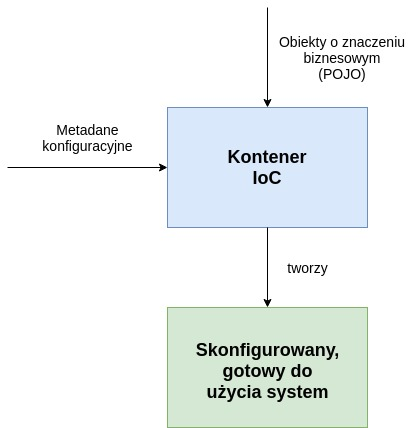
\includegraphics[width=0.55\linewidth]{SpringDiagram1}
		}
		\caption{Kontener Inversion of Control}
		\centering
		\label{fig:inversionOfControl}
	\end{figure}


Odwrócenie sterowania oraz wstrzykiwanie zależności ma kilka bardzo istotnych zalet. Najważniejszą z nich jest zapewnienie luźnego powiązania, ponieważ obiekt nie musi zarządzać zależnościami, znać ich implementację oraz lokalizację. Możemy dzięki temu zmienić implementację zależności bez ingerencji w kod klas, które ją wykorzystują. Testowanie takich obiektów staje się łatwiejsze, ponieważ najczęściej definiujemy zależności poprzez interfejsy lub klasy abstrakcyjne, co pozwala stworzyć atrapę implementacji w testach jednostkowych. Kolejną zaletą tego podejścia jest możliwość łatwego określenia konfiguracji ziarna będącej wzorcem dla stworzenia wielu obiektów. Dzięki adnotacjom możemy wskazać zasięg oraz cykl życia danego ziarna. Domyślnym zachowaniem jest utworzenie tylko jednej instancji zależności zgodnie z wzorcem projektowym Singleton i wstrzyknięcie jej do każdego obiektu zależnego. Istnieje jednak kilka innych możliwości np. określenie ziarna jako prototype w wyniku czego, za każdym wstrzyknięciem kontener tworzy nową instancję. Spring pozwala również na ograniczenie zasięgu ziarna do request, session, application, websocket oraz na stworzenie własnego zasięgu. Poprzez adnotację określamy również cykl życia. Innymi słowy definiujemy jakie akcje mają zostać wykonane w określonych momentach funkcjonowania danego ziarna.





\subsection{Angular 6 framework}
\label{subsec:angularFramework}

W przypadku warstwy prezentacji aplikacji wykorzystany został popularny framework Angular w wersji 6 napisany w języku \textit{TypeScript}. Jest on przeznaczony do tworzenia aplikacji internetowych typu \textit{Single-Page} czyli aplikacji, w której interakcja z użytkownikiem odbywa się przez dynamiczne nadpisywanie obecnej strony zamiast ładowania nowej\cite{ANG01}. Podejście to sprawia, że aplikacja internetowa zachowuję się bardziej jak aplikacja okienkowa zainstalowana na komputerze tzn. obcowanie użytkownika z aplikacją internetową odbywa się bez zakłóceń w postaci przeładowania strony. Szkielet ten jest obecnie aktywnie wspierany i rozwijany przez firmę Google. 
Architektura szkieletu Angular składa się z kilku kluczowych elementów: modułów (\textit{NgModules}), komponentów oraz serwisów. Rodzaj elementu jest określany przez odpowiednie metadane w postaci adnotacji umieszczonych w klasach.

Najważniejszym elementem potrzebnym do budowy aplikacji jest moduł, którego zadaniem jest zebranie powiązanego ze sobą kodu i określenie go jako konkretny, funkcjonalny zestaw. Moduł Angulara różni się od modułu JavaScript tym, że deklaruje kontekst kompilacji dla kilku powiązanych ze sobą komponentów oraz łączy te komponenty z innym, powiązanym kodem napisanym w serwisach tak, aby utworzyć konkretną, funkcjonalną jednostkę. Każda aplikacja ma co najmniej jeden moduł nazwany \mbox{\textit{AppModule}}, który zapewnia mechanizm ładowania przy uruchomieniu aplikacji. Każdy moduł może zaimportować funkcjonalność innego modułu oraz wyeksportować swoją. Zalecaną praktyką jest podzielenie całej aplikacji na kilka modułów \cite{ANG02}, każdy z nich powinien hermetyzować pewną funkcjonalność np. wydzielenie osobnego modułu dotyczącego mechanizmu \textit{routing}. Dzięki temu podejściu projekt skomplikowanej aplikacji jest bardziej czytelny oraz możliwe jest zapewnienie mechanizmu \textit{lazy-loading}, co pozwala na optymalizację wydajności aplikacji poprzez ładowanie konkretnej funkcjonalności dopiero w momencie, gdy jest ona potrzebna. Możemy również w prosty sposób zarządzać zależnościami między modułami oraz podmienić implementacje konkretnego modułu bez dużego wpływu na inne elementy aplikacji.


Następnym elementem aplikacji jest komponent, który definiuje widok połączony z szablonem HTML oraz zawiera dane, logikę biznesową. Każda aplikacja ma co najmniej jeden komponent główny tzw. root, który łączy całą hierarchię komponentów ze strukturą DOM strony. Komponenty mogą również używać serwisów, które zapewniają funkcjonalność nie powiązaną z widokami. Widok komponentu jest zdefiniowany jako szablon podobny do języka HTML oraz jest połączony z klasą TypeScript oznaczoną odpowiednią adnotacją\cite{ANG02}. Wyżej wymieniony szablon oprócz składni HTML zawiera znaczniki charakterystyczne dla Angulara. Pojawia się również kilka przydatnych mechanizmów takich jak powiązanie danych wewnątrz komponentu z danymi w strukturze DOM (ang. \textit{data binding}), przekształcenie danych przed wyświetleniem za pomocą tzw. \textit{pipes} oraz specjalnych dyrektyw do określenia co ma zostać pokazane i kiedy. Przed wyświetleniem widoku Angular rozpoznaje określone dyrektywy oraz powiązania danych, aby na ich podstawie zmienić strukturę DOM.

Ostatnim głównym elementem jest serwis oraz ściśle z nim związany mechanizm wstrzykiwania zależności. Głównym zadaniem serwisu jest rozwiązanie jednego konkretnego zadania, którego logika oraz dane nie są powiązane z konkretnym widokiem. Dzięki temu do jednego serwisu może się odwoływać wiele komponentów, w wyniku czego nie powtarzamy tego samego kodu. Popularnymi zadaniami są np. pobieranie danych z serwera, ich walidacja oraz rejestracja działań wykonywanych przez aplikację\cite{ANG03}. Aby komponent mógł skorzystać z serwisu musi on zostać odpowiednio wstrzyknięty. Dzieje się to poprzez stworzenie specjalnego iniektora (ang. \textit{injector}) dla całej aplikacji oraz kilku dodatkowych podczas początkowego ładowania. Iniektor ten tworzy odpowiednie zależności za pomocą specjalnych dostawców (ang. \textit{provider}), którzy wiedzą jak dana zależność ma zostać stworzona lub dostarczona. Dodatkowo zarządza on kontenerem zależności, dzięki czemu jest w stanie użyć ponownie tej samej instancji w kilku miejscach. Mechanizm wstrzykiwania zależności nie ogranicza się tylko do serwisów, jako zależność może zostać określona np. funkcja, jednak należy pamiętać o zapewnieniu dostawcy. Podczas tworzenia nowej instancji komponentu określone zostają zależności, które dany komponent potrzebuje wzorując się na parametrach konstruktora klasy komponentu. Następnie iniektor sprawdza czy istnieją już instancje potrzebnej zależności. Jeżeli nie istnieje taka instancja odwołuje się do dostawcy w celu stworzenia nowej. Gdy wszystkie zależności są już określone i stworzone, wywołany zostaje konstruktor z nimi jako argumentami.


Warto wspomnieć również o jeszcze jednym bardzo ważnym rozwiązaniu używanym w \mbox{Angular}, czyli \textit{routing}. Odpowiada za niego specjalny moduł \textit{Router}, który zapewnia serwis pozwalający zdefiniować nawigację pomiędzy różnymi stanami, hierarchią, widokami w aplikacji. \textit{Router} mapuje ścieżkę URL tak, aby odwołać się do konkretnego widoku. Użytkownik wykonując różne akcje nie jest przekierowywany do nowej strony, zamiast tego router przechwytuje tą akcję i ładuję konkretny widok. \textit{Router} jest też w stanie określić, czy dany moduł ma zostać załadowany w zależności od stanu aplikacji. Interpretacja ścieżek URL jest określona w specjalnych regułach nawigacyjnych, które wiążą ścieżkę z konkretnym komponentem. Historia nawigacji jest również przechowywana, dzięki czemu możliwa jest nawigacja wstecz/wprzód.


\subsection{PostgreSQL}
\label{subsec:postgreSQL}
Do przechowania informacji o użytkownikach oraz projektach została użyta baza danych \mbox{PostgreSQL}. Jest to relacyjno-obiektowy system bazodanowy oparty na licencji \textit{open-source}, który rozszerza składnie języka SQL o szereg dodatkowych funkcjonalności usprawniających pracę z danymi o skomplikowanej strukturze\cite{POS01}. Na przestrzeni wielu lat zyskał reputację systemu niezawodnego oraz rozszerzalnego głównie za sprawą udokumentowanej architektury, integralności danych, zachowania transakcyjności w postaci właściwości ACID oraz szerokiej społeczności, która nieustannie dostarcza innowacyjne i wydajne rozwiązania.


Główną zaletą tego systemu jest jego bardzo obszerna i treściwa dokumentacja oraz mnogość funkcji rozszerzających standard języka SQL. Pierwsza z dodatkowych funkcjonalności to możliwość określenia przechowywanych danych za pomocą licznych typów wbudowanych lub stworzonych przez programistę. Wbudowanych jest około 40, wśród nich warto wymienić kilka naprawdę przydatnych np. \textit{json/xml}, \textit{inet}, \textit{polygon}, \textit{money}. Następną istotną funkcjonalnością jest zapewnienie integralności danych poprzez możliwość nadania odpowiednich ograniczeń dla danej kolumny np. UNIQUE. Pozwala to na dodatkowe zabezpieczenie przed niepoprawnym zapisem danych. Kolejną bardzo ważna zaletą tego systemu jest skupienie się na wydajności oraz wielowątkowości poprzez liczne systemy wspomagające pracę. Warto wymienić tutaj kilka z nich np. możliwość indeksowania danych w celu szybszego wyszukiwania, optymalizację zapytań do systemu, zapewnienie transakcyjności, współbieżność zapytań typu “read”, partycjonowanie tabel oraz kompilacja wyrażeń w postaci JIT ( ang. \textit{Just-in-time}). Istotną z punktu widzenia bezpieczeństwa aplikacji jest również funkcjonalność związana z uwierzytelnianiem. PostgreSQL zapewnia wbudowane algorytmy szyfrujące takie jak GSSAPI, SSPI, LDAP, SCRAM-SHA-256, które można wykorzystać w przypadku przechowywania wartościowych danych użytkowników np. hasła dostępu. Oprócz wyżej wspomnianych cech Postgres zapewnia również wyjątkową niezawodność poprzez kilka mechanizmów odzyskiwania informacji po awarii oraz zapobiegania jej.

